\section{Building process}
As seen from Figure \ref{Fig:Build_process}, the building process is composed by various phases:
\begin{itemize}
	\item Using an editor, you create the source and header files.
	\item The makefile defines which operations are needed to complete the build and which files have to be build.
	\item The preprocessor analyzes the source code and runs the preprocessor directives: macros, \#defines, ecc.. are expanded in "normal code": the full source is now ready to be compiled and goes in one *.i file. This operation can be seen by stopping the building process with the command \code{g++ -E main.c -o hello.i}
	\item After compiling the *.i files we get the assembly code, another human-readable text file. This output file can be seen by stopping the building process with the command \code{g++ -c hello.c}
	\item The next step is a
\end{itemize}
\begin{figure}[h]
	\centering
	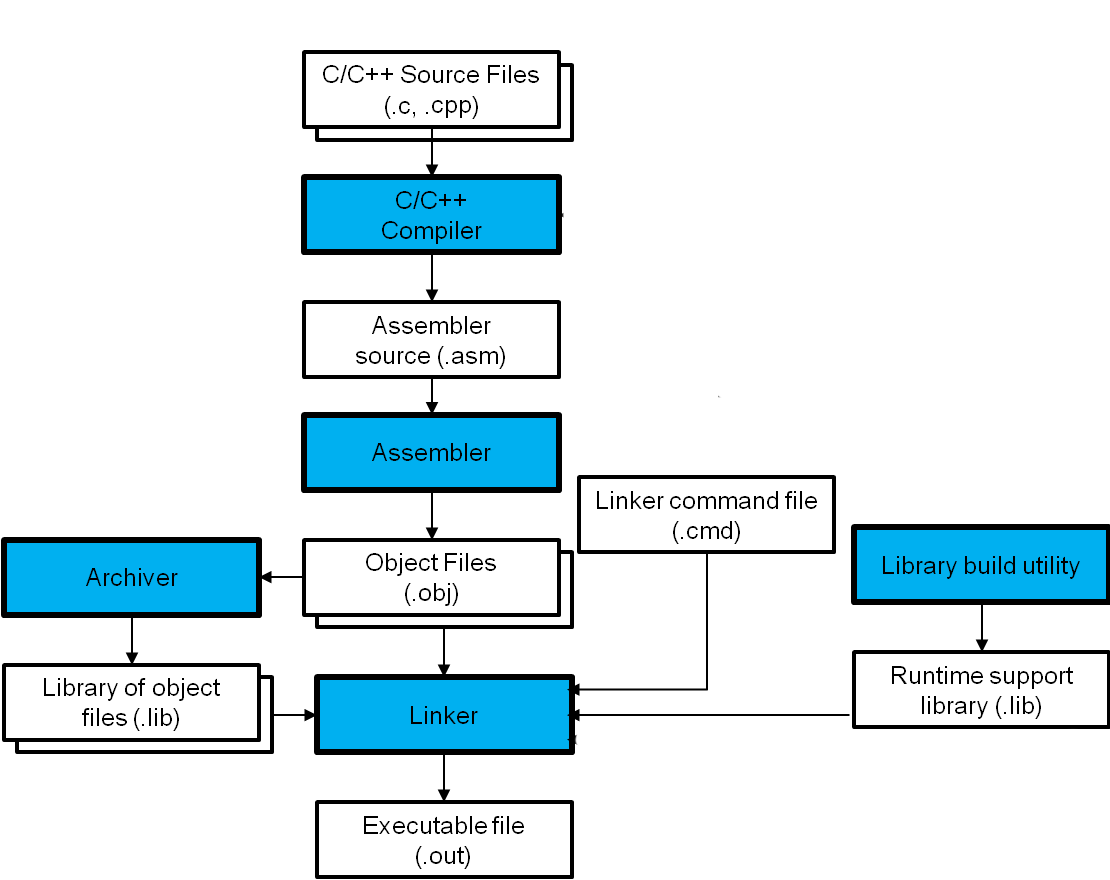
\includegraphics[width=\textwidth]{gfx/build_process}
	
	\caption{Build Process Procedure}
	\label{Fig:Build_process}
\end{figure}